\title{Area, Volume, and Determinants}
\subtitle{\SubTitleName}
\institute[]{\Course}
\author{\Instructor}
\maketitle   


\frame{\frametitle{Topics and Objectives}
\Emph{Topics} \\
\TopicStatement
\begin{itemize}

    \item relationships between area, volume, and determinants
    
\end{itemize}

\vspace{0.5cm}

\Emph{Objectives}\\

\LearningObjectiveStatement

\begin{itemize}

    \item apply determinants to compute the area of a parallelogram, or the volume of a parallelepiped

\end{itemize}

\vspace{0.25cm} 
% Students are not expected to be familiar with Cramer's rule. 

}

%%% FRAME
%\begin{frame}\frametitle{Cramer's Rule, Volume, Linear Transformations}
%
%For a $ n \times n$ matrix $ A = \begin{bmatrix*}[r]
%\vec a_1 & \cdots &\vec  a _{n}
%\end{bmatrix*}$ and any $ \vec b\in \mathbb R ^{n}$.  And for any $ i$, let 
%\begin{equation*}
%A _{i} (\vec b) = 
%\begin{bmatrix*}[r]
%\vec a_1 & \cdots & \vec a _{i-1} & \vec b & a _{i+1} & \cdots & \vec a_n 
%\end{bmatrix*}
%\end{equation*}
%
%
%%%%%%%%%%%%%%%%%%%%%%%%%%%%%%% THEOREM THEOREM THEOREM 
%\begin{center}\begin{tikzpicture} \node [mybox](box){\begin{minipage}{0.80\textwidth} 
%
%Let $ A$ be an invertible $ n \times n $ matrix. For any $ \vec b \in \mathbb R ^{n}$, the unique solution $\vec x$ of the equation $ A \vec x = \vec b$ has the $ i$th entry given by 
%\begin{equation*}
%x_i = \frac { \operatorname {det} A_i (\vec b)} {\operatorname {det} A} , \qquad i=1 ,\dotsc, n. 
%\end{equation*}
%
% \end{minipage}}; \node[fancytitle, right=10pt] at (box.north west) {Theorem Cramer's Rule}; \end{tikzpicture}\end{center}
% %%%%%%%%%%%%%%%%%%%%%%%%%%%%%% THEOREM THEOREM THEOREM
%
%\end{frame}

%\begin{frame}
%
%\textbf{Example.}  For which $ s$ does the system have a unique solution?  Use Cramer's rule to find the solution. 
%\begin{align*}
%3s x_1 - 2 x_2 &=4 \\ -6x_1 + s x_2 &= 1
%\end{align*}
%\end{frame}
%



%\begin{frame}
%The solution to $ A \vec x = e_j$ is the $ j$th column of $ A ^{-1} $.  By Cramer's Rule, the $ i$th entry of $ \vec x $ is 
%\begin{gather*}
%\textup{$(i,j)$th entry of $ A ^{-1} $} = x_i = \frac { \operatorname {det} A (e_j)} {\operatorname {det} A} 
%\\
%\operatorname {det} A (e_j)  = (-1) ^{i+j} A _{jk} = C _{ji}
%\end{gather*}
%where $ C _{ji}$ is the cofactor, and the row/column indices are reversed. 
%
%
%%%%%%%%%%%%%%%%%%%%%%%%%%%%%%% THEOREM THEOREM THEOREM 
%\begin{center}\begin{tikzpicture} \node [mybox](box){\begin{minipage}{0.80\textwidth} 
%
%\begin{equation*}
%A ^{-1} = \frac 1 {\operatorname {det} A} 
%= 
%\begin{bmatrix*}[r]
%C _{11}  & C _{21} & \cdots & C _{n1} 
%\\
%C _{12} &  C _{22} & \cdots & C _{n2} 
%\\
%\vdots  & \vdots & \ddots & \vdots 
%\\
%C _{1n} & C _{2n} & \cdots & C _{nn}
%\end{bmatrix*}
%\end{equation*}
%
% \end{minipage}}; \node[fancytitle, right=10pt] at (box.north west) {Theorem: Cramer's Rule (Second Version)}; \end{tikzpicture}\end{center}
% %%%%%%%%%%%%%%%%%%%%%%%%%%%%%% THEOREM THEOREM THEOREM
%
%\end{frame}
  


\begin{frame}\frametitle{Area and Determinants}

    Recall that in $\mathbb R^2$, determinants can give us the area of a parallelogram.
    
    \pause 
    \begin{center}
    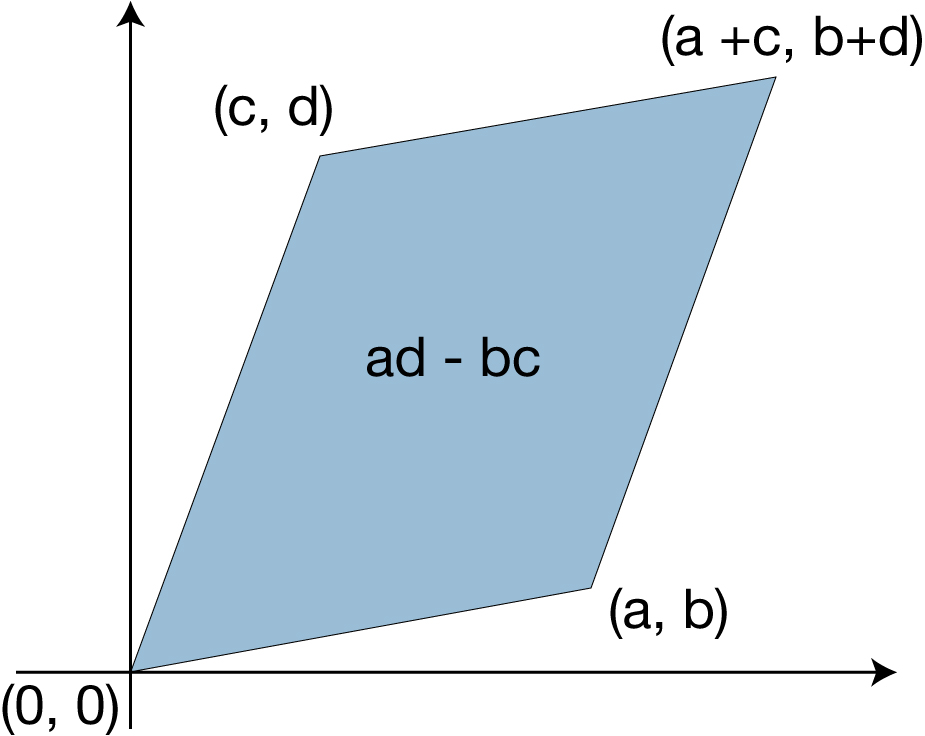
\includegraphics[width=.4\textwidth]{Chapter3/images/image002.jpg} 
    \end{center}
    
    \pause 
    area of parallelogram =  $| \det \spalignmat{a c;b d} | = | ad - bc |$. 

\end{frame}



\begin{frame}\frametitle{Area and Determinants}


 \Emph{Key Geometric Fact (which works in any dimension).} 
 The area of the parallelogram spanned by two vectors $ \vec a, \vec b$ is equal to the area spanned 
by $ \vec a , c\vec a + \vec b$, for any scalar $ c$.   
 
\begin{center}
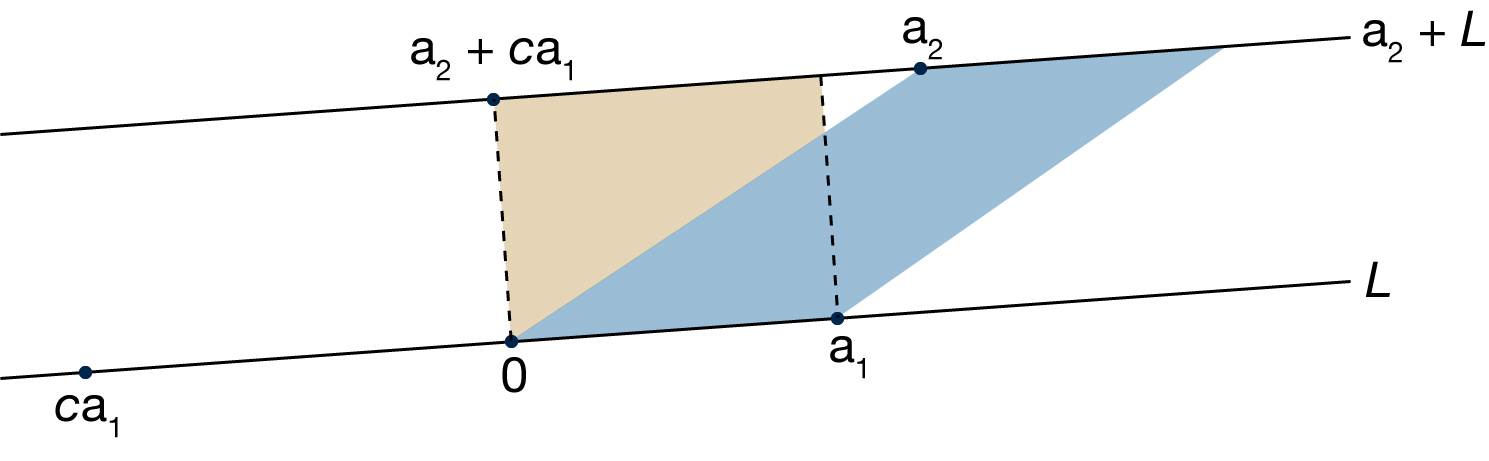
\includegraphics[width=0.7\textwidth]{Chapter3/images/image003.jpg} 
\end{center}

\end{frame}




\begin{frame}\frametitle{Example: Area of a Parallelogram}
    Calculate the area of the parallelogram determined by the points $(-2, -2), (0, 3), (4, -1)  ,(6, 4)$, shown in (a). 
    
    \begin{center}
    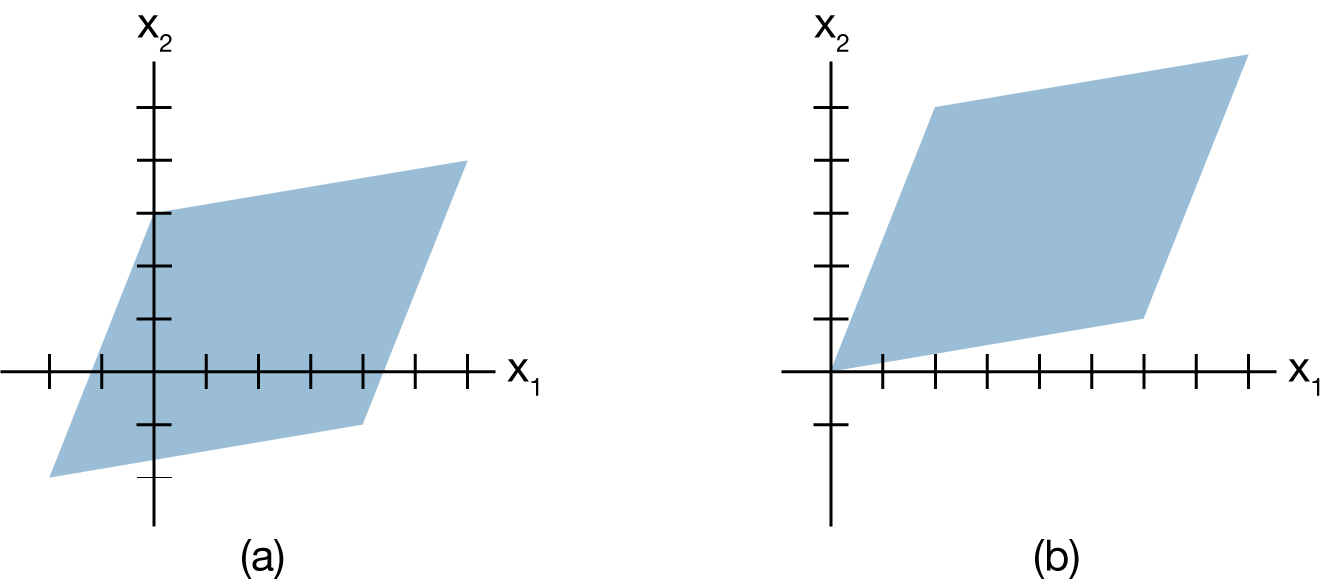
\includegraphics[width=0.6\textwidth]{Chapter3/images/image001.jpg}  
    \end{center}
    
    Note that translating a region in $\mathbb R^2$ does not change its area. 
\end{frame}


\begin{frame}\frametitle{Determinants of $n\times n$ Matrices}

\begin{center}\begin{tikzpicture} \node [mybox](box){\begin{minipage}{0.80\textwidth} \vspace{2pt}

The volume of the parallelpiped spanned by the columns of an $n\times n$ matrix $ A$ is $ \lvert  \operatorname {det} A\rvert $. 

 \end{minipage}}; \node[fancytitle, right=10pt] at (box.north west) {Theorem}; \end{tikzpicture}\end{center}


\end{frame}


\begin{frame}\frametitle{Example: Volume of a Parallelepiped}

    Any $3 \times  3$ matrix $ A$ can be transformed into a diagonal matrix using row operations that do not change 
    $ \lvert  \operatorname {det} (A)\rvert $. 
    
    \vspace{12pt}
    \begin{center}
    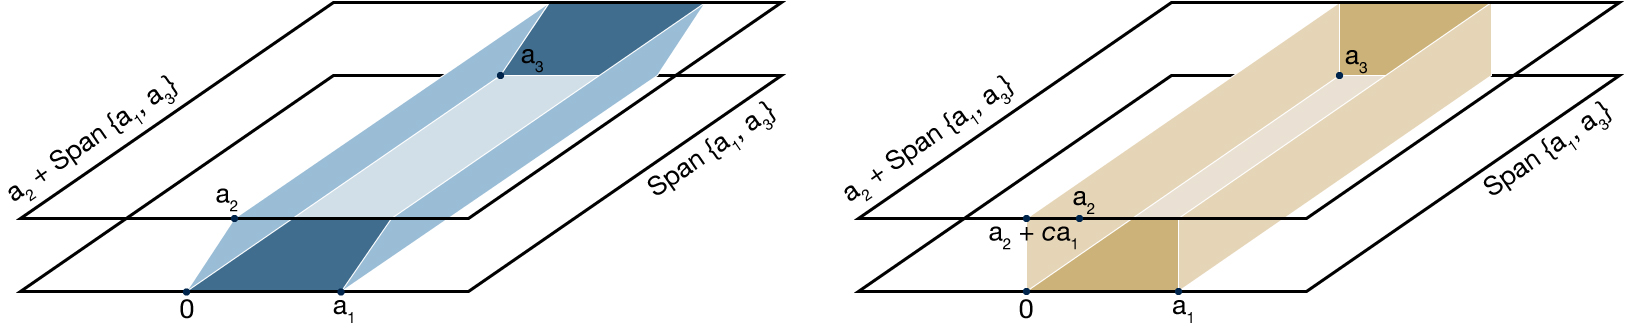
\includegraphics[width=\textwidth]{Chapter3/images/image004.jpg} 
    \end{center}

\end{frame}



\begin{frame}\frametitle{Example: Volume of a Parallelepiped}

    Compute the volume of the parallelepiped that has one vertex at the origin, and adjacent vertices at $(2,0,0)$, $(1,3,0)$, and $(0,1,4)$.  

\end{frame}


\frame{\frametitle{Summary}

    \SummaryLine \vspace{4pt}
    \begin{itemize}\setlength{\itemsep}{8pt}
        \item using determinants to compute the area of a parallelogram, or the volume of a parallelepiped
    \end{itemize}
    
}








